\section{Synthetic numerical experiments}
\label{sec:numerical-experiments}

For the recovery and geometric tests, we generate separator observations from known sites and weights. The generating power diagram supplies both separator positions and a reference set of neighboring pairs. We first ask which weight information can be recovered from these observations. Exact data provide a numerical control; separate experiments then remove observations or corrupt their values. This separates information that is absent from information that is present but noisy (Section~\ref{subsec:numerical-accuracy}).

We next test two situations in which agreement with separator data can give an incomplete picture of the geometry. Periodic observations may specify the wrong site images, and deliberately altered separator positions may fail to admit a common set of weights. We examine image identity and realized adjacency alongside numerical error (Section~\ref{subsec:numerical-geometry}). Finally, we add candidate pairs to the generating neighbor graph and test whether the optional refinement of Section~\ref{subsec:workflow-active-mask} improves the fitted separators or the selection of pairs (Section~\ref{subsec:numerical-refinement}).

These comparisons use different references for different questions. Error against clean generating separators measures recovery from corrupted data; error against deliberately imposed targets measures agreement with those targets. Geometric scores compare either all realized adjacencies or the selected candidate observations, as specified below. The fitting and tessellation calculations use \texttt{pyvoro2} 0.6.3 \cite{Pyvoro2_063}. The scripts, configurations and numerical results are deposited in the \texttt{powerfit} 1.0.0 archive \cite{PowerfitArchive2026}. The experiment labels A--H identify its records; detailed configurations and evaluation conventions are collected in \ref{app:numerical-protocols}.

\subsection{Recovery from exact, incomplete, and noisy observations}
\label{subsec:numerical-accuracy}

We begin with compatible observations extracted from a power diagram (Experiment A). Sixteen tests cover two and three dimensions, periodic and nonperiodic domains, and connected and disconnected observation graphs. The largest recorded separator root mean square error (RMSE) is $1.31\times10^{-14}$ in normalized-coordinate units. Thus the observed weight differences are recovered to numerical precision. When the observation graph is disconnected, however, the relative offsets of its components remain undetermined. Choosing these offsets can change competition between cells in different components, even while preserving every observed difference. The archived tests include a case in which some requested faces are consequently absent from the reconstructed diagram.

Experiment C examines this loss of information by randomly deleting observations \emph{without adding noise}. Within each remaining connected component, the observations still determine all relative weights. What is lost is the relation between different components. We display this distinction using two errors against the known generating weights. The \emph{globally aligned} error removes one common additive shift, whereas the \emph{componentwise aligned} error removes a separate shift on each observed component. Componentwise alignment uses the generating weights for evaluation; it does not recover the missing offsets from the retained observations.

Figure~\ref{fig:missing-observations} shows the resulting profiles for 128 sites in each dimension, selected from the 2,470 archived runs. As observations are removed, the componentwise error remains near numerical precision even where the graphs are disconnected. In the two-dimensional tests retaining half the observations, for example, all ten graphs are disconnected: the median globally aligned weight RMSE is $3.53\times10^{-5}$, while its componentwise counterpart is $1.42\times10^{-15}$. A small error on the information retained within components therefore coexists with uncertainty in the full weight vector. The connected fraction provides the corresponding diagnostic for global identifiability.

\begin{figure}[!tbp]
\centering
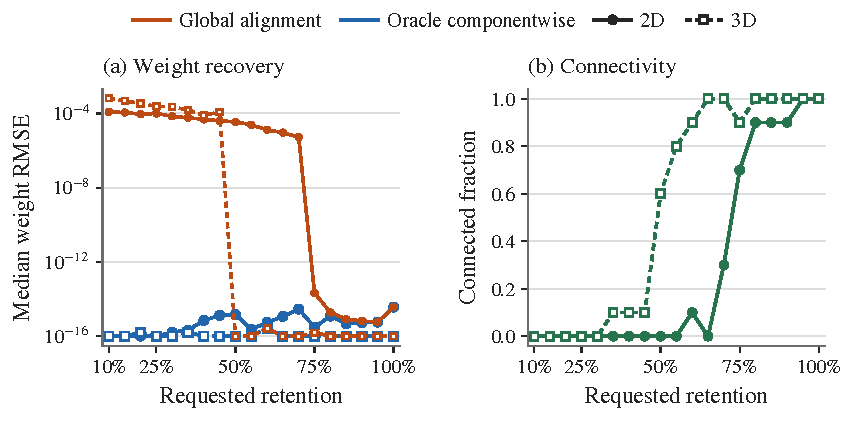
\includegraphics[width=\linewidth]{figures/figure_C_identifiability.pdf}
\caption{Missing observations without added noise (Experiment C), for $n=128$ in two and three dimensions. The horizontal coordinate is the requested retention fraction. Left: medians of per-run weight RMSE after one global alignment or separate componentwise alignments to the known generating weights. Values below $10^{-16}$ are floored for display on the logarithmic axis. Right: fraction of connected observation graphs. Each retention setting uses ten independently generated runs, so the curves are sampled profiles rather than nested deletion trajectories or universal connectivity thresholds.}
\label{fig:missing-observations}
\end{figure}

Observation error introduces a different difficulty even when the correct pair graph is known. Experiment B compares quadratic and Huber fitting under three noise conditions: Gaussian perturbations, Laplace perturbations, and sparse outliers on a Gaussian background. Accuracy is measured against the untouched generating separators, rather than against the corrupted fitting targets. The tested outlier cases show a modest benefit from Huber fitting. For example, in the two-dimensional setting with a nominal $5\%$ outlier fraction, the mean clean-reference separator RMSE is $0.00809$ for quadratic fitting and $0.00755$ for Huber fitting, in normalized-coordinate units. The benefit is not uniform across the Gaussian and Laplace settings; the noise levels, threshold and complete configuration are given in \ref{app:synthetic-noise}.

Hard restrictions raise a separate question: can they be satisfied simultaneously? As a short control, Experiment D correctly classifies all 30 generated three-observation cases as feasible or contradictory. It uses a dedicated experimental difference-constraint checker, distinct from the production fitting precheck; its construction is described in \ref{app:synthetic-controls}.

\subsection{Separator agreement and geometric realization}
\label{subsec:numerical-geometry}

A separator observation in a periodic system identifies both a site pair and a particular image. Experiment F asks what happens when that image information is wrong. In the noiseless control with the generating image shifts supplied, separator errors are near numerical precision and all requested faces are realized. Deliberately incorrect supplied shifts remain fixed during fitting: adjusting the weights does not revise the observation's image identity. A realized face at another image can therefore expose a mismatch that the fitted separator value alone does not resolve.

F also tests a separate image-selection procedure. It removes the image labels, chooses nearest images, and optionally revises them using uniquely realized shifts. In the three-dimensional tests, the revised choices all agree with their realized-image diagnostics, but only a fraction $0.924$ agree with the generating shifts. Geometric self-consistency is therefore insufficient to establish the correct periodic-image identity. This image-selection procedure is separate from the optional observation-set refinement, which retains the supplied shifts. Repeated stripped-label inputs and the exact scoring conventions are documented in \ref{app:synthetic-images}.

Experiment G instead keeps the generating diagram's neighbor pairs and alters their separator targets. Structured pair-dependent changes are added with amplitude $\eta$; the resulting targets need not be representable by one weight per site. The \emph{type-cycle} law encodes cyclic preferences among three site types, while the \emph{local-context} law uses contrasts in local neighbor spacing; their definitions are given in \ref{app:synthetic-mismatch}. We fit those targets and then compare the \emph{entire realized adjacency graph} with the generating graph. This tests whether closer agreement with local separator positions also preserves the reference neighbor relations. We summarize pair agreement by F1, the harmonic mean of precision (the fraction of realized pairs belonging to the reference) and recall (the fraction of reference pairs realized).

Figure~\ref{fig:model-mismatch} compares fitting accuracy and geometric recovery throughout the tested range of structured perturbations. The fit has lower error against the imposed separator targets than the ordinary Voronoi midpoint baseline at every tested amplitude. At $\eta=0$, when the targets come from a generating power diagram, the fitted diagrams have higher mean realized-graph F1; as the imposed targets are perturbed, this mean advantage reverses for both perturbation laws. The data at different amplitudes use independent configurations, so the trends are not trajectories of individual diagrams or universal mismatch thresholds.

\begin{figure}[!tbp]
\centering
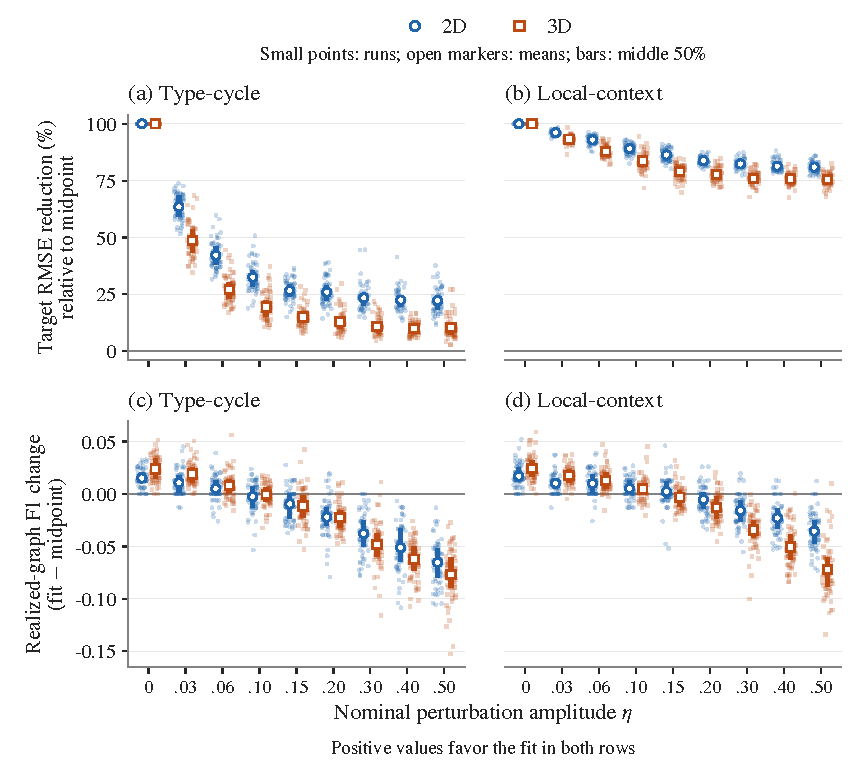
\includegraphics[width=\linewidth]{figures/figure_G_mismatch.pdf}
\caption{Target fitting and realized adjacency under structured mismatch (Experiment G). Columns show the two perturbation laws; circles and squares denote two and three dimensions. Each amplitude/dimension/law group contains 60 runs from two geometry families and three site counts. Top: percentage reduction in separator RMSE relative to midpoints, evaluated on the imposed fitting targets. Bottom: fitted minus midpoint F1 for the \emph{entire realized adjacency graph}, relative to the generating graph; positive values favor the fit in both rows. Faint points show runs, open markers their arithmetic means, and bars the middle 50\% of values (not confidence intervals). Nominal amplitudes are equally spaced for display, and instances at different amplitudes are independent. At $\eta=0.5$, target-coordinate clipping affects on average $38.25\%$ of type-cycle targets (\ref{app:synthetic-mismatch}).}
\label{fig:model-mismatch}
\end{figure}

At $\eta=0.2$, all 24 configuration groups have lower mean target RMSE after fitting, but also lower mean realized-graph F1. For example, among 60 two-dimensional type-cycle runs, the mean target RMSE is $0.109$ for the fit versus $0.147$ for midpoints, while mean realized-graph F1 is $0.961$ versus $0.983$. These are means of per-run scores. The midpoint baseline is itself an admissible equal-weight fit, and the same imposed targets enter both fitting and its error evaluation; lower in-sample target error therefore does not establish better recovery of the generating geometry. The perturbation laws and numerical protocol are detailed in \ref{app:synthetic-mismatch}.



\subsection{Optional refinement: benefits and failures}
\label{subsec:numerical-refinement}

The previous tests know which pairs supplied the generating diagram's separators. Experiments E and H add other pairs as candidates and ask whether the optional refinement can identify a more useful subset of observations. Every candidate set contains all generating neighbor pairs. In E, their targets receive small random errors, while the additional candidates receive approximate midpoint targets. H combines the enlarged candidate set with structured separator changes of the kind used in G.

We compare a one-pass fit using every candidate observation with the refined fit. For pair selection, the one-pass result selects candidates whose requested faces are realized; refinement selects the observations in its returned active set. Precision, recall and F1 compare these selections with the fixed set of generating neighbor pairs. Thus the scores concern selection among the candidates, rather than all adjacencies of the final diagram. Separator RMSE is evaluated on that same fixed reference-pair set, against clean generating separators in E and the imposed, potentially incompatible targets in H. All separator errors are in normalized-coordinate units.

\begin{table}[!htbp]
\centering
\footnotesize
\setlength{\tabcolsep}{4pt}
\caption{One-pass and refined fits in E and H. Values are arithmetic means of paired per-run scores. RMSE uses the fixed generating neighbor pairs, with clean targets in E and imposed targets in H; F1 scores the selected candidate observations. Counts classify the paired changes: lower RMSE or higher F1 is better. H includes the 72 positive-mismatch comparisons, excluding $\eta=0$.}
\label{tab:refinement-paired}
\begin{tabular}{@{}llrrrrr@{}}
\toprule
Study & Score & One pass & Refined & Better & Tied & Worse \\
\midrule
E (20) & RMSE & 0.00790 & 0.00385 & 19 & 0 & 1 \\
 & F1 & 0.99253 & 0.99479 & 4 & 15 & 1 \\
\cmidrule(lr){1-7}
H ($\eta>0$, 72) & RMSE & 0.13118 & 0.13422 & 70 & 0 & 2 \\
 & F1 & 0.96755 & 0.96701 & 19 & 32 & 21 \\
\bottomrule
\end{tabular}
\end{table}

In E, refinement approximately halves the mean error against clean separators, while the already high mean pair-selection F1 changes little (Table~\ref{tab:refinement-paired}). All 20 refinements reach the implemented self-consistency condition. The main benefit in these instances is therefore more accurate separator positions; it is not a substantial improvement in pair selection.

\Needspace{10\baselineskip}
H shows why frequent improvements and a favorable mean need not coincide. Error decreases in 70 of the 72 positive-mismatch comparisons, yet its mean increases because of a severe adverse case. One run worsens from $0.1266$ to $0.6929$ with unchanged pair-selection F1 and stops after a previously seen active set recurs. Across all 96 H refinements, including zero mismatch, 85 stop on the implemented self-consistency test and 11 after an active set recurs. The recorded final inner fits have optimal status, but the recurrence of an active set does not establish convergence of the outer updates. The error, selected pairs and stopping outcome must therefore be assessed separately.

% SOURCE A--D: results/{exact_recovery,noise_robustness,missing_data_manuscript,infeasible}/.
% SOURCE F/G: results/{periodic,model_mismatch}/ and their experimental generators.
% SOURCE E/H: results/{active_set,supergraph_mismatch}/runs.csv; paired
% by seed and configuration in scripts/check_manuscript_tables.py. H uses
% eta>0; stopping counts use all 96 refinements. The absolute tie tolerance
% is 1e-12 on unrounded score changes. See manuscript/README.md evidence map.
% Figure C: scripts/plot_editorial_figures.py reads the frozen runs.csv;
% no simulation, fitting or solver result is recomputed.
